\documentclass[tikz]{standalone}

\usepackage{tikz}
\usetikzlibrary{positioning, fit, shapes.geometric, arrows}

\tikzstyle{block} = [draw, fill=white, rectangle,
    minimum width=0.5cm, minimum height=0.5cm]

\begin{document}
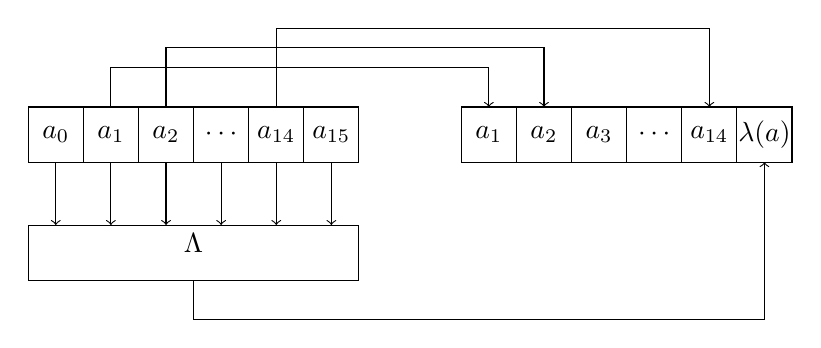
\begin{tikzpicture}[
    node distance=0pt,
    every node/.style = {draw, minimum size=7mm, inner sep=0pt, outer sep=0pt}
]
    \node (a0) {$a_0$};
    \node [right=of a0.east] (a1) {$a_1$};
    \node [right=of a1.east] (a2) {$a_2$};
    \node [right=of a2.east] (ai) {$\cdots$};
    \node [right=of ai.east] (a14) {$a_{14}$};
    \node [right=of a14.east] (a15) {$a_{15}$};
    \node [fit={(a0) (a15)}, yshift=-1.5cm] (lambda) {$\Lambda$};

    \node [right of=a15, node distance=2cm] (b0) {$a_1$};
    \node [right=of b0.east] (b1) {$a_2$};
    \node [right=of b1.east] (b2) {$a_3$};
    \node [right=of b2.east] (bi) {$\cdots$};
    \node [right=of bi.east] (b14) {$a_{14}$};
    \node [right=of b14.east] (b15) {$\lambda(a)$};

    \draw[->] (a1.north) |- ++(0,0.5) -| (b0.north);
    \draw[->] (a2.north) |- ++(0,0.75) -| (b1.north);
    \draw[->] (a14.north) |- ++(0,1) -| (b14.north);

    \draw[->] (a0.south) -- (a0.south |- lambda.north);
    \draw[->] (a1.south) -- (a1.south |- lambda.north);
    \draw[->] (a2.south) -- (a2.south |- lambda.north);
    \draw[->] (ai.south) -- (ai.south |- lambda.north);
    \draw[->] (a14.south) -- (a14.south |- lambda.north);
    \draw[->] (a15.south) -- (a15.south |- lambda.north);

    \draw[->] (lambda.south) |- ++(0,-0.5) -| (b15.south);
\end{tikzpicture}
\end{document}